% !TeX program = lualatex
% Lualatex is important to render Fira fonts; with pdflatex it's just the regular one
\documentclass[12pt]{beamer}

\usetheme{metropolis}
\usepackage{appendixnumberbeamer}

% adjust the background to be completely white
\setbeamercolor{background canvas}{bg=white}

\usepackage{booktabs}
\usepackage[scale=2]{ccicons}

\usepackage{pgfplots}
\usepgfplotslibrary{dateplot}

% typeset mathematics on serif
\usefonttheme[onlymath]{serif}

% better bibliography using biber as backend
\usepackage[natbib=true,backend=biber,style=authoryear-icomp,maxbibnames=30,maxcitenames=3,uniquelist=false,giveninits=true,doi=false,url=true,dashed=false,isbn=false]{biblatex}
% shared bibliogrphy
\addbibresource{../dl4nlp-bibliography.bib}
% disable "ibid" for repeated citations
\boolfalse{citetracker}

% TODOs
\usepackage{todonotes}
\let\todox\todo
\renewcommand\todo[1]{\todox[inline]{#1}}

\definecolor{76abdf}{RGB}{118, 171, 223}

\setbeamercolor{frametitle}{bg=76abdf, fg=white}

\usepackage{xspace}
\newcommand{\themename}{\textbf{\textsc{metropolis}}\xspace}

% POS tags
\newcommand*\POS[1]{\textsubscript{\texttt{#1}}} % tag with part of speech

% parse tree
\usepackage{qtree}

% NNEts
\usepackage{tikz}
\usetikzlibrary{matrix, positioning, calc}

\tikzset{
	neuron/.style={
		draw,
		circle,
		inner sep=0pt,
		minimum width=0.75cm
	},
	layer/.style={
		matrix of nodes,
		nodes={neuron},
		row sep={between origins, 1.2cm}, %1.5cm in general, 2.5cm for backprop task
		nodes in empty cells
	}
}

% for derivatives, https://tex.stackexchange.com/a/412442
\usepackage{physics}


\title{Deep Learning for Natural Language Processing}
\subtitle{Lecture 2 -- Machine Learning Basics}
\date{April 20, 2021}
\author{Dr.\ Ivan Habernal}
\institute{Trustworthy Human Language Technologies  \hfill 
\includegraphics[height=.8cm]{img/logo-trusthlt.pdf} \\
Department of Computer Science\\
Technical University of Darmstadt \hfill \texttt{www.trusthlt.org} }
%\titlegraphic{\hfill }

\begin{document}

\maketitle


%\begin{frame}{Table of contents}
%  \setbeamertemplate{section in toc}[sections numbered]
%  \tableofcontents[hideallsubsections]
%\end{frame}

%\section{Administrative course issues}

\begin{frame}{This lecture}
	
Machine Learning Principles

\begin{itemize}
	\item Train/dev/test split
	\item Evaluation
	\item Loss functions
\end{itemize}

Learning goals

\begin{itemize}
	\item Understand ML/DL foundations
\end{itemize}

\end{frame}

\begin{frame}{Notation}
	Vectors in linear algebra are columns, for example $\mathbf{x} \in \mathbb{R}^3$
	
$$
\mathbf{x} = 
\begin{pmatrix}
x_1 \\
x_2 \\
x_3
\end{pmatrix} \qquad \text{(bold face, lower case)}
$$

We treat them as a row vector by transposing, for example $\mathbf{x}^\intercal = (x_1, x_2, x_3)$ --- which is a matrix $\mathbb{R}^{1 \times 3}$

\emph{Caveat:} 1-D array (a list of numbers) is sometimes considered a vector, so dealing with dimensions might be quite messy
	
\end{frame}

\begin{frame}{Notation}
Matrices are upper-case bold, for example $\mathbf{Z} \in \mathbb{R}^{2 \times 3}$

$$
\mathbf{Z} =
\begin{pmatrix}
z_{1,1} & z_{1,2} & z_{1,3} \\
z_{2,1} & z_{2,2} & z_{2,3} \\
\end{pmatrix}
$$

Scalars are ordinary lower case letters, for example

$$
a, b, c \in \mathbb{R}
$$

\end{frame}

\begin{frame}{Notation ambiguity}
A dot $\cdot$ means multiple things, depending on context
	
Simple scalar multiplication, for example $a \cdot b$

$$\cdot : \mathbb{R} \times \mathbb{R} \to \mathbb{R}$$

Dot product $\mathbf{x} \cdot \mathbf{y} = \sum_{i = 1}^{n} x_i y_i$

$$\cdot : \mathbb{R}^n \times \mathbb{R}^n \to \mathbb{R}$$

Matrix-matrix (matrix-vector/vector-matrix) multiplication, for example $\mathbf{x} \cdot \mathbf{W}$ or $\mathbf{Y} \cdot \mathbf{Z}$

$$\cdot : \mathbb{R}^{m \times n} \times \mathbb{R}^{n \times p} \to \mathbb{R}^{m \times p}$$
	
\end{frame}

\begin{frame}{Derivatives}
	
Derivative of function $f(x)$ is denoted as $\dv{f}{x}$ (rarely as $f'$)

Partial derivates of a function of several real variables $f(x_1, \dots, x_n)$ we use

$$
\pdv{f}{x_i}
$$

The gradient is then a row vector of partial derivatives

$$
\nabla f = \left( \pdv{f}{x_1}, \dots, \pdv{f}{x_n}  \right)
$$
	
\end{frame}

\begin{frame}{Notation}
Vector-matrix multiplication

- What is $\mathbf{x} \cdot \mathbf{W}$ if $\mathbf{x} \in \mathbb{R}^{1 \times n}$ and $\mathbf{W} \in \mathbb{R}^{n \times d}$?

Cosine similarity

- For two vectors $\mathbf{x}, \mathbf{y}$, their \emph{cosine similarity} is defined as

$$
\frac{\mathbf{x} \cdot \mathbf{y}}{\norm{\mathbf{x}} \norm{\mathbf{y}}} =
\frac{\sum_i x_i y_i}{\sqrt{\sum_i {x_i^2}} \cdot \sqrt{\sum_i{y_i^2}}} \qquad \in \mathopen[ 0, 1\mathclose]
$$

Functions applied element-wise to vectors, e.g., $f: \mathbb{R}^{1 \times n} \to \mathbb{R}^{1 \times n}$

$$
f(\mathbf{x}) = (f(x_i), \dots, f(x_n))
$$

\end{frame}

\section{Supervised Machine Learning basics}

\begin{frame}{Problem setup}
	
We have $N$ labeled \textbf{data points} (or examples) as tuples

$$
(\mathbf{x}_1, y_1), (\mathbf{x}_2, y_2), \dots, (\mathbf{x}_N, y_N)
$$

where $y_n$ is the "truth" or "gold label" of $\mathbf{x}_n$.

We have a \textbf{model} parametrized by $\theta$ that outputs $y$ (or $\hat{y}$)

$$
\hat{y} = f_{\theta}(\mathbf{x})
$$
	
We specify a \textbf{loss function}, for example

$$
\frac{1}{N} \sum_{i = 1}^{N} \left( y_i - f_{\theta}(\mathbf{x}_i) \right)^2
$$
	
\end{frame}

\begin{frame}{Learning}
	
Our goal is to find such parameters $\theta$ that minimize the loss

- In other words, our model "fits" the training data "better"


\metroset{block=fill}
\begin{block}{Overfitting}
If our model is sufficiently "rich" (huge number of parameters), it could minimize the loss by \textbf{remembering} our training data perfectly $\to$ Not the goal of learning!
\end{block}

	
\end{frame}


\begin{frame}{Generalization}
The actual goal of machine learning is to \textbf{generalize} well on previously unseen data

\bigskip

Evaluating generalization?

- Split dataset into training and test

- Models must perform well on test data (hidden during learning)

\end{frame}


\begin{frame}{Regularization and hyperparameters}

Regularization for preventing overfitting by putting constraints on $\theta$ (e.g., penalizing large parameter values)

\bigskip

Hyperparameters?

- Learning rate, early stopping, batch size, etc.

- Hyperparameter tuning: Split training data into training and development
	
\end{frame}


\begin{frame}{ML Basics}
	
Three major components of a machine learning system
	
- Data,

- Models

- Learning
	
	
\end{frame}

\begin{frame}{Supervised learning problem: Data}

Dataset is a set of input-label tuples (labeled examples)

$$
\{(\mathbf{x}_1, y_1), \dots,  (\mathbf{x}_n, y_n), \dots,  (\mathbf{x}_N, y_N)\}
$$

- $N$ denotes the number of examples in a dataset, we index the examples with lowercase $n = 1, \dots, N$.

\bigskip

- Each input $\mathbf{x}_n$ is a $D$-dimensional vector of real numbers, which are called features, attributes, or covariates

- Label $y_n$ associated with input vector $\mathbf{x}_n$

Compact representation of the dataset inputs: $\mathbf{X} \in \mathbb{R}^{N \times D}$
	
\end{frame}

\begin{frame}{Models as Functions}

\emph{Predictor} is a function that, when given a particular input example produces an output

$$
f: \mathbb{R}^{D} \to \mathbb{R}
$$

- For illustration, we predict single real (regression)

- In classification we typically predict a probability distribution over categories, e.g.

$$
f: \mathbb{R}^{D} \to \mathbb{R}^{|C|}
$$

where $|C|$ is the number of classes, and the (arbitrary) mapping is

$$
C =
\begin{cases}
0  & \quad \text{Sport}\\
1  & \quad \text{Politics}\\
2  & \quad \text{Business}
\end{cases}
$$

\end{frame}


\begin{frame}{Models as Functions}
	
Classification models typically predict a probability distribution over categories ($|C|$ is the number of classes)
	
	$$
	f: \mathbb{R}^{D} \to \mathbb{R}^{|C|}
	$$
	
For example
	
$$
C =
\begin{cases}
0  & \quad \text{Sport}\\
1  & \quad \text{Politics}\\
2  & \quad \text{Business}
\end{cases}
$$
	
$$
f: \mathbb{R}^{D} \to \underbrace{(0.01, 0.82, 0.17)}_{\sum = 1.0}
$$

	
\end{frame}


\begin{frame}{Learning is Finding Parameters}

\metroset{block=fill}
\begin{block}{The goal of learning is to}

- find a model and its corresponding parameters

- such that the resulting predictor will perform well on unseen data
\end{block}


Conceptually three distinct algorithmic phases when discussing machine learning algorithms

\begin{enumerate}
\item Prediction or inference
\item Training or parameter estimation
\item Hyperparameter tuning or model selection	
\end{enumerate}

\end{frame}

\begin{frame}{Hypothesis Class of Functions}

Supervised learning on dataset $\{(\mathbf{x}_1, y_1), \dots,  (\mathbf{x}_N, y_N)\}$; $x_n \in \mathbb{R}^D$

Estimate a predictor parametrized by $\theta$ (e.g., a vector of $\mathbb{R}$ parameters)

$$
f(\cdot, \theta): \mathbb{R}^D \to \mathbb{R}
$$

We hope to "find" "good" parameters $\theta^*$ so that we "fit" the data well

$$
f(\mathbf{x}_n, \theta^*) \approx y_n \qquad \text{for all } n = 1, \dots, N
$$

Notation: let $\hat{y_n} = f(\mathbf{x}_n, \theta^*)$ represent predictor's output

\end{frame}

\begin{frame}{Loss Function for Training}

What does it mean to fit the data "well"?

We need to specify a \textbf{loss function}

$$
\ell(\underbrace{y_n}_{\text{True label}}, \underbrace{\hat{y_n}}_{\text{Predictor's output}}) \to \underbrace{\mathbb{R}^{+}}_{\text{"Loss"}}
$$

- representing how much error we have made on this particular prediction

Our goal for finding a good parameter vector $\theta^*$ is to \textbf{minimize the average loss} on the set of $N$ training examples


\end{frame}

\begin{frame}{Independent and identically distributed}

Assumption: Our dataset  $\{(\mathbf{x}_1, y_1), \dots,  (\mathbf{x}_N, y_N)\}$ is \textbf{Independent and identically distributed (I.I.D)}

- Two data points $(\mathbf{x}_i, y_i)$ and $(\mathbf{x}_j, y_j)$ do not statistically depend on each other

- Implication: We can use the \textbf{empirical mean} of the loss on the training data ("empirical risk")

$$
\mathbf{R}_{\mathrm{emp}} (f, \mathbf{X}, \mathbf{y}) = 
\frac{1}{N} \left[ \ell(y_1, \hat{y_1}) + \dots + \ell(y_N, \hat{y_N}) \right] =
\frac{1}{N} \sum_{i = 1}^{N} \ell(y_i, \hat{y_i}) 
$$

\end{frame}

\begin{frame}{Loss example: Squared Loss}

$$
\ell(y_n, \hat{y_n}) = (y_n - \hat{y_n})^2
$$

Minimizing empirical risk

$$
\min_{\theta} \frac{1}{N} \sum_{i = 1}^{N} (y_i - f(\mathbf{x}, \theta))^2
$$


\end{frame}

\begin{frame}{Expected risk}
	
Not interested in a predictor that only performs well on the training data

We seek a predictor that performs well (has low risk) on unseen test data.

That is, finding a predictor $f$ (with parameters fixed) that minimizes the \textbf{expected risk}

$$
\mathbf{R}_{\mathrm{true}} (f) = \mathbb{E}_{\mathbf{x}, y}
\left[ \ell (y, f(\mathbf{x}))   \right]
$$

$y$ is the label; $f(\mathbf{x})$ is the prediction based on example $x$


The expectation is over the (infinite) set of all possible data and labels

\end{frame}


\begin{frame}{Expected risk}
	
Minimizing the \textbf{expected risk}

$$
\mathbf{R}_{\mathrm{true}} (f) = \mathbb{E}_{(\mathbf{x}, y) \sim P} \left[ \ell (y, f(\mathbf{x}))   \right] = 
\int_{\mathcal{X} \times \mathcal{Y}}  \ell (y, f(\mathbf{x})) P(\mathbf{x},y) \mathrm{ d}\mathbf{x} \mathrm{d}y
$$
	

\emph{The expectation is over the (infinite) set of all possible data and labels.}

\begin{itemize}
	\item How to estimate expected risk from (finite) data?
	\item How to change training to generalize well?
\end{itemize}

	



Empirical risk minimization = Approximately minimizing expected risk

Simulate unseen data: hold out a proportion of the whole dataset
	
\end{frame}





\begin{frame}{Generalization}

We're interested in generalization performance, not how predictor works on training data

We always split our data:
	
- The \textbf{training set} is used to fit the model

- The \textbf{test set} is used to evaluate generalization performance
	
\textbf{Test set} not seen by the machine learning algorithm during training
	

	
\end{frame}


\begin{frame}{Overfitting}

Empirical risk minimization can lead to \textbf{overfitting}

\emph{The predictor fits too closely to the training data and does not generalize well to new data}

- Having very small average loss on the training set but large average loss on
the test set?

- Tends to occur when we have little data and a complex hypothesis class
	

\end{frame}

\begin{frame}{Overfitting}

Predictor $f$ (with parameters fixed); overfitting occurs when the risk estimate from the training data 

$$
\mathbf{R}_{\mathrm{emp}} (f, \mathbf{X}_{\mathrm{train}}, \mathbf{y}_{\mathrm{train}})
$$

\textbf{underestimates} the expected risk  $\mathbf{R}_{\mathrm{true}} (f)$.
 
Since we estimate the expected risk  $\mathbf{R}_{\mathrm{true}} (f)$ by using the empirical risk on the test set 


$$
\mathbf{R}_{\mathrm{emp}} (f, \mathbf{X}_{\mathrm{test}}, \mathbf{y}_{\mathrm{test}})
$$

if the test risk is much larger than the training risk, this is an indication of overfitting.
	
\end{frame}


\begin{frame}{Cross-validation}


\textbf{K-fold cross-validation} partitions the data into $K$ chunks

$K - 1$ of which form the training set $\mathcal{R}$

The last chunk serves as the validation set $\mathcal{V}$

\bigskip

\tikzstyle{box} = [rectangle, draw, black, text width=1.5cm]
\tikzstyle{train} = [fill=blue!10]
\tikzstyle{test} = [fill=red!10]

\begin{figure}
\begin{scriptsize}
\begin{tikzpicture}[node distance=0.5cm]
\node (f10) [] {Fold 1};
\node (f11) [box, train, below of=f10] {Train};
\node (f12) [box, train, below of=f11] {Train};
\node (f13) [box, train, below of=f12] {Train};
\node (f14) [box, train, below of=f13] {Train};
\node (f15) [box, test, below of=f14] {Test};

\node (f20) [right=1.6cm, right of=f10] {Fold 2};
\node (f21) [box, train, below of=f20] {Train};
\node (f22) [box, train, below of=f21] {Train};
\node (f23) [box, train, below of=f22] {Train};
\node (f24) [box, test, below of=f23] {Test};
\node (f25) [box, train, below of=f24] {Train};

\node (f30) [right=1.6cm, right of=f20] {Fold 3};
\node (f31) [box, train, below of=f30] {Train};
\node (f32) [box, train, below of=f31] {Train};
\node (f33) [box, test, below of=f32] {Test};
\node (f34) [box, train, below of=f33] {Train};
\node (f35) [box, train, below of=f34] {Train};

\node (f40) [right=1.6cm, right of=f30] {Fold 4};
\node (f41) [box, train, below of=f40] {Train};
\node (f42) [box, test, below of=f41] {Test};
\node (f43) [box, train, below of=f42] {Train};
\node (f44) [box, train, below of=f43] {Train};
\node (f45) [box, train, below of=f44] {Train};

\node (f50) [right=1.6cm, right of=f40] {Fold 5};
\node (f51) [box, test, below of=f50] {Test};
\node (f52) [box, train, below of=f51] {Train};
\node (f53) [box, train, below of=f52] {Train};
\node (f54) [box, train, below of=f53] {Train};
\node (f55) [box, train, below of=f54] {Train};
\end{tikzpicture}
\end{scriptsize}
\caption{Example of 5-fold CV}
\end{figure}

\end{frame}

\begin{frame}{Cross-validation}


For each partition $k$, the training data $\mathcal{R}^{(k)}$ produces a predictor $f^{(k)}$

It is then applied to validation set $\mathcal{V}^{(k)}$ to compute the empirical risk $\mathbf{R}(f^{(k)}, \mathcal{V}^{(k)})$

\bigskip

Cross-validation approximates the expected generalization error

$$
\mathbb{E}_{\mathcal{V}} \left[ \mathbf{R}(f, \mathcal{V}) \right] \approx
\frac{1}{K} \sum_{k = 1}^{K} \mathbf{R}(f^{(k)}, \mathcal{V}^{(k)})
$$
	
\end{frame}

\begin{frame}{Hyper-parameter optimization}

Training data can be also split to two parts: Training and Development set

Development set used for optimizing hyper-parameters

\textbf{Nested cross-validation}

- For model selection

\tikzstyle{box} = [rectangle, draw, black, text width=1.5cm]
\tikzstyle{train} = [fill=blue!10]
\tikzstyle{dev} = [fill=yellow!10]
\tikzstyle{test} = [fill=red!10]


\begin{figure}
	\begin{scriptsize}
		\begin{tikzpicture}[node distance=0.5cm]
\node (f10) [] {Fold $k$};
\node (f11) [box, train, below of=f10] {Train};
\node (f12) [box, train, below of=f11] {Train};
\node (f13) [box, train, below of=f12] {Train};
\node (f14) [box, dev, below of=f13] {Validation};
\node (f15) [box, test, below of=f14] {Test};
	

\node (f20) [right=1.6cm, right of=f10] {};
\node (f21) [box, train, below of=f20] {Train};
\node (f22) [box, train, below of=f21] {Train};
\node (f23) [box, dev, below of=f22] {Validation};
\node (f24) [box, train, below of=f23] {Train};

\node (f30) [right=1.6cm, right of=f20] {\emph{... inner loop ...}};
\node (f31) [box, train, below of=f30] {Train};
\node (f32) [box, dev, below of=f31] {Validation};
\node (f33) [box, train, below of=f32] {Train};
\node (f34) [box, train, below of=f33] {Train};

\node (f40) [right=1.6cm, right of=f30] {};
\node (f41) [box, dev, below of=f40] {Validation};
\node (f42) [box, train, below of=f41] {Train};
\node (f43) [box, train, below of=f42] {Train};
\node (f44) [box, train, below of=f43] {Train};



		\end{tikzpicture}
	\end{scriptsize}
	\caption{Example of 5-fold nested CV}
\end{figure}




\end{frame}


\begin{frame}{Evaluation}
	
	
We often use \textbf{accuracy} on the test data to evaluate our model performance:

- How many instances are correctly classified divided by the number of instances in the test set
	
- However, there are other plausible evaluation	measures:
	
When your outputs are continuous:

- Squared distance (MSE), cosine, correlation, etc.
	
Say, your output is a sequence:

- Could use edit distance, for instance
	
\end{frame}

\begin{frame}{Evaluation}

Two systems predict whether a patient has a rare disease $Q$. Which system is better?

\begin{table}
	\begin{footnotesize}
		\begin{tabular}{l|rr}
			& Prediction is Q & Prediction is not Q \\ \hline
			Patient has Q & 0 & 10 \\
			Patient has not Q & 1 & 1004 \\
		\end{tabular}
	\end{footnotesize}
	\caption{System A}
\end{table}

\begin{table}
	\begin{footnotesize}
		\begin{tabular}{l|rr}
			& Prediction is Q & Prediction is not Q \\ \hline
			Patient has Q & 4 & 6 \\
			Patient has not Q & 5 & 1000 \\
		\end{tabular}
	\end{footnotesize}
	\caption{System B}
\end{table}

Both systems have accuracy 1004/1015 = 0.99
	
\end{frame}



\begin{frame}{Terminology}
	
	Confusion matrix for binary classification
	
	\begin{table}
		\begin{footnotesize}
			\begin{tabular}{l|rr}
				& Prediction is Q & Prediction is not Q \\ \hline
				Truth is Q & True positive (\textbf{TP}) & False negative (\textbf{FN}) \\
				Truth is not Q & False positive (\textbf{FP}) & False negative (\textbf{FN}) 
			\end{tabular}
		\end{footnotesize}
	\end{table}
	
	
\end{frame}




\begin{frame}{Precision and recall}
	
For Class \emph{Disease}

- System B has \textbf{precision} of $4/9 = 0.444$

- and recall of $4/10 = 40$

- System A has precision of $0$ and recall of $0$

\bigskip

For Class \emph{No Disease}

- both systems are very close:

• Precision A: 1004/1014, Pr B: 1000/1006

• Recall A: 1004/1005, Rec B: 1000/1005

\end{frame}

\begin{frame}{F-measure}
	
When there are more than two classes, precision and recall for class $k$ are defined as

$$
\mathrm{P}_k = \frac{C_{k,k}}{ \sum_{i} C_{i,k}}
\qquad
\mathrm{R}_k =  \frac{C_{k,k}}{ \sum_{i} C_{k,i}}
$$

where $C$ is a confusion matrix as above

\bigskip

From precision and recall, compute the $F_1$-score 

$$
F_1 = \frac{2 \mathrm{P} \mathrm{R}}{\mathrm{P} + \mathrm{R}}
$$

	
\end{frame}


\begin{frame}{Evaluation – F1 measure}
	
For two or more classes, we typically compute the F1-score of each class and then combine this in an overall score:

\begin{itemize}
	\item For example, averaging all the F1 scores
	\item There are several ways of averaging with different names (e.g. micro F1 vs. macro F1)
\end{itemize}

Very relevant reading:

\begin{scriptsize}


\fullcite{Forman.Scholz.2009.SIGKDD}

\fullcite{Sokolova.Lapalme.2009}

\end{scriptsize}
	
\end{frame}


\begin{frame}{Other evaluation metrics in NLP}
	
Evaluating \textbf{language generation} is not trivial\footnote{\begin{scriptsize}\fullcite{caglayan-etal-2020-curious}\end{scriptsize}}
	
\begin{itemize}
\item Machine Translation (MT)
\begin{itemize}
	\item BLEU is based on n-gram matches between the candidate and reference sentences
	\begin{itemize}
		\item but increase in BLEU does not always indicate an improvement in quality
	\end{itemize}
\end{itemize}
\item Summarization
\begin{itemize}
	\item 	ROUGE-L: longest common sub-sequences between
	the candidate and references, i.e. a set of shared words with similar order even if not contiguous
\end{itemize}
\end{itemize}
	
\vspace{1em }
	
\end{frame}


\section{Loss functions}


\begin{frame}{Loss over multi-dimensional output}

We already introduced loss function as  $\ell : \mathbb{R} \times \mathbb{R} \to \mathbb{R}^+$

$$
\ell(\underbrace{y_n}_{\text{True label}}, \underbrace{\hat{y_n}}_{\text{Predictor's output}}) \to \underbrace{\mathbb{R}^{+}}_{\text{"Loss"}}
$$

For a neural network with multi-dimensional output ($M$ output neurons), we extend the loss to $\ell : \mathbb{R}^M \times \mathbb{R}^M \to \mathbb{R}^+$


$$
\ell(\underbrace{\mathbf{y}_n}_{\text{True label}}, \underbrace{\hat{\mathbf{y}_n}}_{\text{Predictor's output}}) \to \underbrace{\mathbb{R}^{+}}_{\text{"Loss"}}
$$

Where $\mathbf{y}_n = (y_{n,1}, y_{n, 2}, \dots, y_{n,m}, \dots, y_{n,M})$ or if $n$ is clear from context simply $\mathbf{y} = (y_{1}, y_{2}, \dots, y_{m}, \dots, y_{M})$



\end{frame}


\begin{frame}{Multi-dimensional square loss}

For $M = 1$, we had\footnote{For each example $n$; here dropping out $n$ from the formula for clarity}

$$
\ell(y, \hat{y}) = (y - \hat{y})^2
$$

For multiple dimensions

$$
\ell(\mathbf{y}, \hat{\mathbf{y}}) =  (\mathbf{y}_m - \hat{\mathbf{y}}_m)^2 = \sum_{m = 1}^{M} (y_m - \hat{y_m})^2
$$


\end{frame}


\begin{frame}{Background: K-L divergence}
	
Also known as \emph{relative entropy}

Let $Y$ and $\hat{Y}$ be categorical random variables over same categories, with probability distributions $P(Y)$ and $Q(\hat{Y})$
	
	\begin{align*}
	\mathbb{D}(P(Y) || Q(\hat{Y})) &= \mathbb{E}_{P(Y)} \left[ \log \frac{P(Y)}{P(\hat{Y})} \right] \\
	&= \mathbb{E}_{P(Y)} \left[ \log P(Y) - \log P(\hat{Y}) \right] \\
	&= \mathbb{E}_{P(Y)} \left[ \log P(Y)\right] - \mathbb{E}_{P(Y)} \left[ \log P(\hat{Y}) \right] \\
	&= - \mathbb{E}_{P(Y)} \left[ \log \frac{1}{P(Y)}\right] - \mathbb{E}_{P(Y)} \left[ \log P(\hat{Y}) \right] \\
	&= - \mathbb{H}_{P} (Y)  - \mathbb{E}_{P(Y)} \left[ \log P(\hat{Y}) \right] \\
	\end{align*}
	

	
\end{frame}


\begin{frame}{Cross-entropy loss}

Labels as categorical probability distributions

\begin{align*}
\mathbb{D}(P(Y) || Q(\hat{Y})) &= - \mathbb{H}_{P} (Y)  - \mathbb{E}_{P(Y)} \left[ \log P(\hat{Y}) \right] \\
\end{align*}

$\mathbb{H}_{P} (Y)$ does not depend on predictions $\hat{Y}$ so we only care about $- \mathbb{E}_{P(Y)} \left[ \log P(\hat{Y}) \right]$; Let $P(Y = m) = y_m$

\begin{align*}
\ell(\mathbf{y}, \hat{\mathbf{y}}) &= 
- \mathbb{E}_{P(Y)} \left[ \log P(\hat{Y}) \right]
= - \sum_{m = 1}^{M} P(Y = m) \log P(\hat{Y} = m)\\
&=-  \sum_{m = 1}^{M} y_m \log (\hat{y}_m) 
\end{align*}


\end{frame}


\begin{frame}{Examples}

$\mathbf{y}_n$ is $n$-th example true label, $\hat{\mathbf{y}}_n$ is $n$-th example prediction

$$\mathbf{y}_n = (0, 1, 0, 0) \qquad \hat{\mathbf{y}}_n = (0.25, 0.3, 0.4, 0.05)$$

Cross-entropy loss $\ell(\mathbf{y}, \hat{\mathbf{y}}) = \sum_{m} y_m \log (\hat{y}_m)$

$\ell(\mathbf{y}, \hat{\mathbf{y}}) = - \log 0.3 \approx 1.737$

\bigskip

Square loss $\ell(\mathbf{y}, \hat{\mathbf{y}}) =  \sum_{m} (y_m - \hat{y_m})^2$

$\ell(\mathbf{y}, \hat{\mathbf{y}}) = (0-0.25)^2 + (1 - 0.3)^2 + (0-0.4)^2 + (0 - 0.05)^2$


\end{frame}

\begin{frame}{Comparison of square loss and cross-entropy loss}

$$
\mathbf{y}_n = (1, 0) \qquad \hat{\mathbf{y}}_n = (z, 1 - z) \qquad z \in  \mathbb{R} : \langle 0, 1 \rangle
$$

\begin{columns}
	
	\begin{column}{0.4\linewidth}
		
		Square loss
		
		$$\ell(\mathbf{y}_n, \hat{\mathbf{y}_n}) = 2(1 - z)^2$$
		
		\bigskip
		
		Cross-entropy loss
		
		$$\ell(\mathbf{y}_n, \hat{\mathbf{y}_n}) = - \log z$$
		
	\end{column}
	
	\begin{column}{0.6\linewidth}
		
		\begin{figure}
			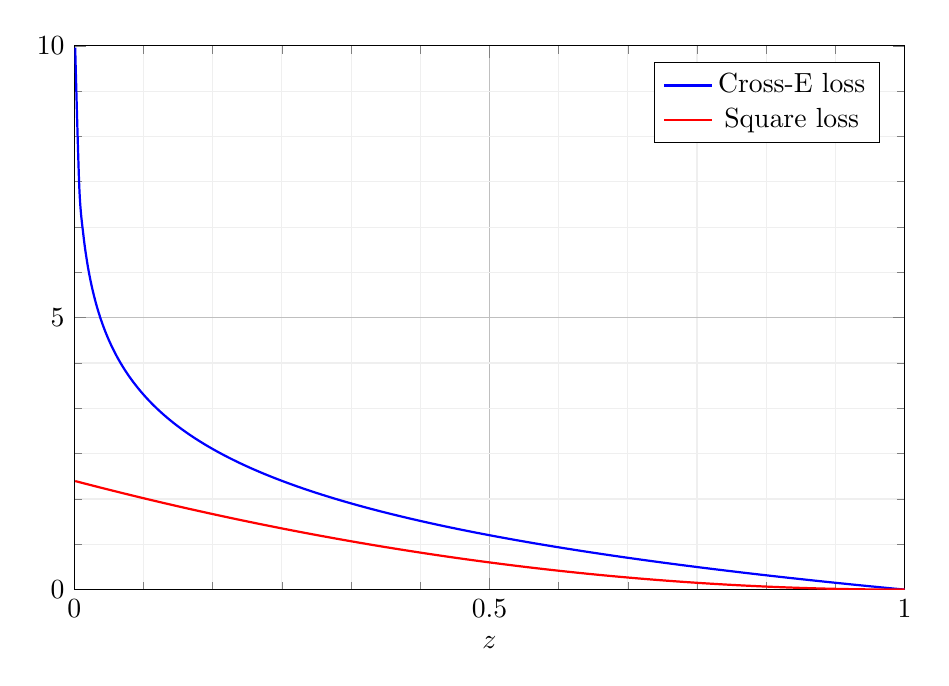
\begin{tikzpicture}
			
			\begin{axis}[
			xmin = 0, xmax = 1,
			ymin = 0, ymax = 10,
			xtick distance = 0.5,
			ytick distance = 5,
			grid = both,
			minor tick num = 5,
			major grid style = {lightgray},
			minor grid style = {lightgray!25},
			width = \textwidth,
			height = 0.7\textwidth,
			legend pos = north east,
			xlabel={$z$},
			]
			
			\addplot[
			domain = 0.001:1,
			samples = 200,
			smooth,
			thick,
			blue,
			] {-log2(x)};
			
			\addplot[
			domain = 0.001:1,
			samples = 200,
			smooth,
			thick,
			red,
			] {2*(1-x)^2};
			
		
			
			\legend{
				Cross-E loss,
				Square loss, 
			}
			
			
			\end{axis}
			
			\end{tikzpicture}
			\caption{Comparison of losses as function of $z$ for a concrete example}
		\end{figure}
	\end{column}
\end{columns}

\end{frame}


\begin{frame}{Summary}
	
"Bread \& butter" of machine learning

\begin{itemize}
	\item Notation
	\item Goals of supervised machine learning
	\item Scenarios for training and testing, cross-validation
	\item Evaluation
	\item Loss functions
\end{itemize}

\end{frame}

\begin{frame}{Further suggested reading}

Chapter 8 of \fullcite{Deisenroth.et.al.2021.book}

Chapter 5 of \fullcite{Goodfellow.et.al.2016.book}

For probabilistic treatment Chapter 16 of \fullcite{Koller.Friedman.2009.book}


\end{frame}

%\begin{frame}[allowframebreaks]{References}
%\printbibliography
%  \bibliography{demo}
%  \bibliographystyle{abbrv}
%\end{frame}

\end{document}

